\documentclass[tikz,border=12pt]{standalone}
\usepackage{xcolor}
\usepackage{amsmath,amssymb}
\usepackage{times}
\usetikzlibrary{shapes.geometric, arrows.meta, positioning, calc, fit, backgrounds, shadows, fadings}

\definecolor{ieeeBlue}{RGB}{0, 98, 155}
\definecolor{ieeeNavy}{RGB}{0, 40, 85}
\definecolor{ieeeLightBlue}{RGB}{235, 243, 250}
\definecolor{ieeeCyan}{RGB}{0, 163, 196}
\definecolor{ieeeGrayBox}{RGB}{248, 249, 250}
\definecolor{ieeeAccentGreen}{RGB}{0, 138, 90}
\definecolor{ieeeAccentAmber}{RGB}{217, 130, 43}
\definecolor{ieeeAccentRed}{RGB}{198, 40, 40}

\begin{document}
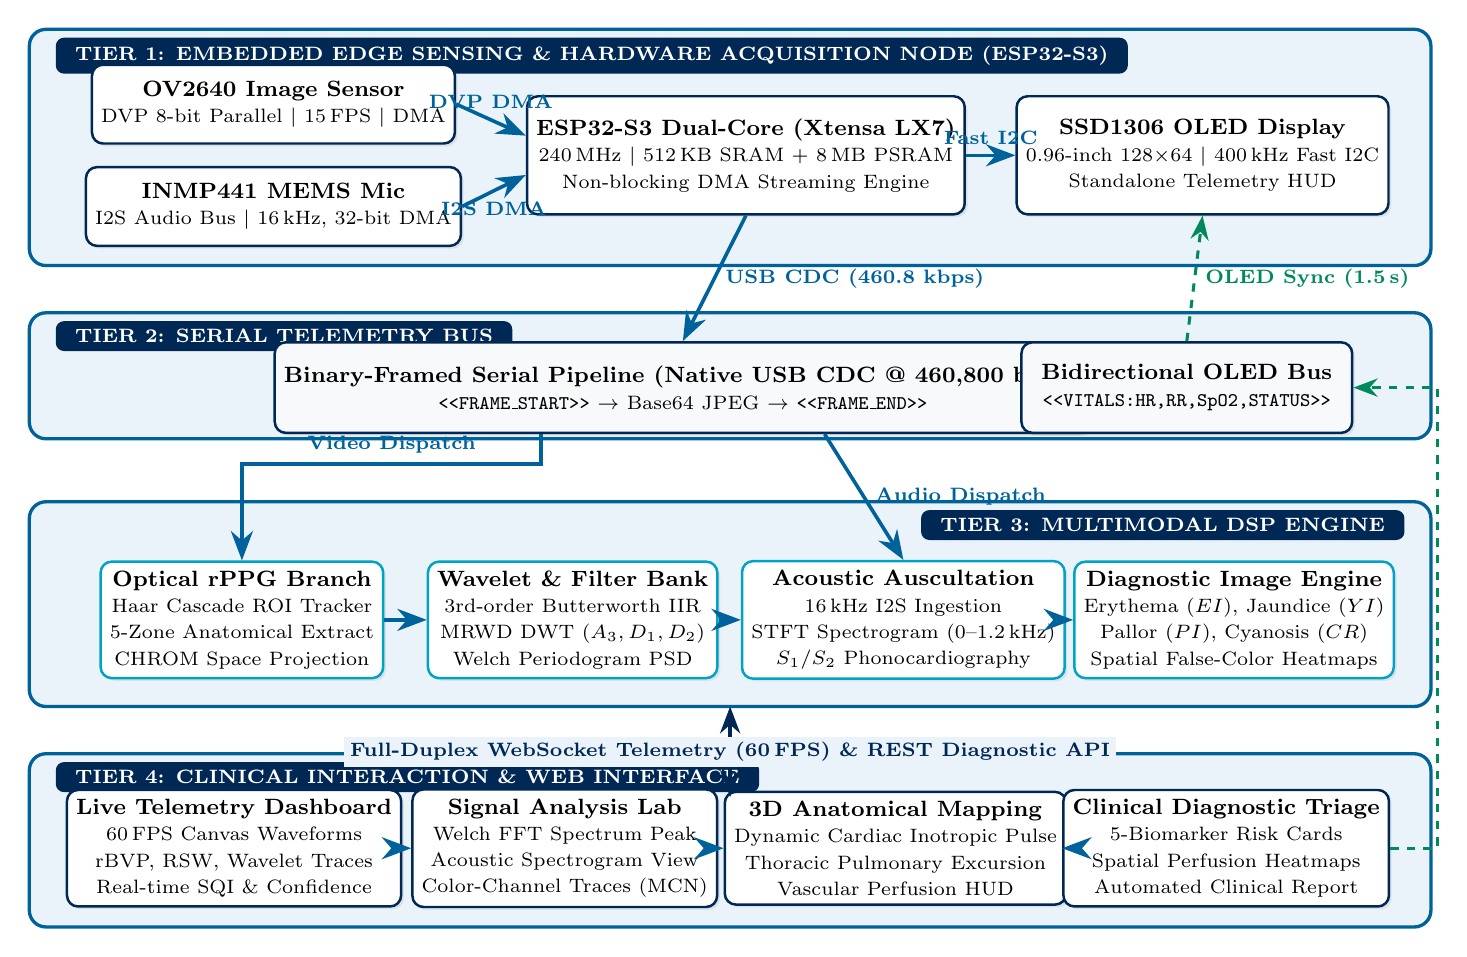
\begin{tikzpicture}[
    tierBox/.style={draw=ieeeBlue, fill=ieeeLightBlue, rounded corners=6pt, line width=1.2pt, inner sep=6pt},
    compBox/.style={draw=ieeeNavy, fill=white, rounded corners=4pt, line width=0.9pt, align=center, font=\footnotesize, minimum height=1.15cm, drop shadow={opacity=0.15, shadow xshift=1pt, shadow yshift=-1pt}},
    dspBox/.style={draw=ieeeCyan, fill=white, rounded corners=4pt, line width=0.9pt, align=center, font=\footnotesize, minimum height=1.25cm, drop shadow={opacity=0.15, shadow xshift=1pt, shadow yshift=-1pt}},
    bannerTab/.style={draw=none, fill=ieeeNavy, text=white, font=\bfseries\scriptsize, rounded corners=3pt, inner xsep=7pt, inner ysep=3.0pt},
    dataArrow/.style={-{Stealth[scale=1.2]}, line width=1.3pt, color=ieeeBlue},
    bidirArrow/.style={{Stealth[scale=1.1]}-{Stealth[scale=1.1]}, line width=1.3pt, color=ieeeNavy},
    syncArrow/.style={-{Stealth[scale=1.1]}, line width=1.1pt, dashed, color=ieeeAccentGreen}
]

% ================= TIER 1 =================
\node[tierBox, minimum width=17.8cm, minimum height=3.0cm] (tier1) at (0, 7.8) {};
\node[bannerTab, anchor=north west] at ([xshift=0.35cm, yshift=-0.12cm] tier1.north west) {TIER 1: EMBEDDED EDGE SENSING \& HARDWARE ACQUISITION NODE (ESP32-S3)};

\node[compBox, minimum width=4.0cm, minimum height=1.0cm] (cam) at (-5.8, 8.35) {
    \textbf{OV2640 Image Sensor}\\
    \scriptsize DVP 8-bit Parallel $\vert$ 15\,FPS $\vert$ DMA
};

\node[compBox, minimum width=4.0cm, minimum height=1.0cm] (mic) at (-5.8, 7.05) {
    \textbf{INMP441 MEMS Mic}\\
    \scriptsize I2S Audio Bus $\vert$ 16\,kHz, 32-bit DMA
};

\node[compBox, minimum width=4.6cm, minimum height=1.5cm] (mcu) at (0.2, 7.7) {
    \textbf{ESP32-S3 Dual-Core (Xtensa LX7)}\\
    \scriptsize 240\,MHz $\vert$ 512\,KB SRAM + 8\,MB PSRAM\\
    \scriptsize Non-blocking DMA Streaming Engine
};

\node[compBox, minimum width=4.2cm, minimum height=1.5cm] (oled) at (6.0, 7.7) {
    \textbf{SSD1306 OLED Display}\\
    \scriptsize 0.96-inch 128$\times$64 $\vert$ 400\,kHz Fast I2C\\
    \scriptsize Standalone Telemetry HUD
};

% Direct non-crossing data links in Tier 1
\draw[dataArrow] (cam.east) -- node[above, font=\scriptsize\bfseries\color{ieeeNavy}] {DVP DMA} ([yshift=0.25cm]mcu.west);
\draw[dataArrow] (mic.east) -- node[below, font=\scriptsize\bfseries\color{ieeeNavy}] {I2S DMA} ([yshift=-0.25cm]mcu.west);
\draw[dataArrow] (mcu.east) -- node[above, font=\scriptsize\bfseries\color{ieeeNavy}] {Fast I2C} (oled.west);

% ================= TIER 2 =================
\node[tierBox, minimum width=17.8cm, minimum height=1.6cm] (tier2) at (0, 4.9) {};
\node[bannerTab, anchor=north west] at ([xshift=0.35cm, yshift=-0.12cm] tier2.north west) {TIER 2: SERIAL TELEMETRY BUS};

\node[compBox, minimum width=7.2cm, fill=ieeeGrayBox] (usbStream) at (-0.6, 4.75) {
    \textbf{Binary-Framed Serial Pipeline (Native USB CDC @ 460,800 baud)}\\
    \scriptsize \texttt{<<FRAME\_START>>} $\rightarrow$ Base64 JPEG $\rightarrow$ \texttt{<<FRAME\_END>>}
};

\node[compBox, minimum width=4.2cm, fill=ieeeGrayBox] (oledSync) at (5.8, 4.75) {
    \textbf{Bidirectional OLED Bus}\\
    \scriptsize \texttt{<<VITALS:HR,RR,SpO2,STATUS>>}
};

% Direct vertical links between Tier 1 and Tier 2
\draw[dataArrow] (mcu.south) -- node[right, font=\scriptsize\bfseries\color{ieeeNavy}] {USB CDC (460.8 kbps)} (usbStream.north);
\draw[syncArrow] (oledSync.north) -- node[right, font=\scriptsize\bfseries\color{ieeeAccentGreen}] {OLED Sync (1.5\,s)} (oled.south);

% ================= TIER 3 =================
\node[tierBox, minimum width=17.8cm, minimum height=2.6cm] (tier3) at (0, 2.0) {};
\node[bannerTab, anchor=north east] at ([xshift=-0.35cm, yshift=-0.12cm] tier3.north east) {TIER 3: MULTIMODAL DSP ENGINE};

\node[dspBox, minimum width=3.3cm] (rppgCore) at (-6.2, 1.8) {
    \textbf{Optical rPPG Branch}\\
    \scriptsize Haar Cascade ROI Tracker\\
    \scriptsize 5-Zone Anatomical Extract\\
    \scriptsize CHROM Space Projection
};

\node[dspBox, minimum width=3.3cm] (waveletCore) at (-2.0, 1.8) {
    \textbf{Wavelet \& Filter Bank}\\
    \scriptsize 3rd-order Butterworth IIR\\
    \scriptsize MRWD DWT ($A_3, D_1, D_2$)\\
    \scriptsize Welch Periodogram PSD
};

\node[dspBox, minimum width=3.3cm] (acoustCore) at (2.2, 1.8) {
    \textbf{Acoustic Auscultation}\\
    \scriptsize 16\,kHz I2S Ingestion\\
    \scriptsize STFT Spectrogram (0--1.2\,kHz)\\
    \scriptsize $S_1/S_2$ Phonocardiography
};

\node[dspBox, minimum width=3.3cm] (diagCore) at (6.4, 1.8) {
    \textbf{Diagnostic Image Engine}\\
    \scriptsize Erythema ($EI$), Jaundice ($YI$)\\
    \scriptsize Pallor ($PI$), Cyanosis ($CR$)\\
    \scriptsize Spatial False-Color Heatmaps
};

% Clean links from Tier 2 to Tier 3 (well clear of the Tier 3 banner on right)
\draw[dataArrow] ([xshift=-1.8cm]usbStream.south) -- ++(0,-0.38) -| node[above, pos=0.25, font=\scriptsize\bfseries\color{ieeeNavy}] {Video Dispatch} (rppgCore.north);
\draw[dataArrow] ([xshift=1.8cm]usbStream.south) -- node[right, font=\scriptsize\bfseries\color{ieeeNavy}] {Audio Dispatch} (acoustCore.north);
\draw[dataArrow] (rppgCore.east) -- (waveletCore.west);
\draw[dataArrow] (waveletCore.east) -- (acoustCore.west);
\draw[dataArrow] (acoustCore.east) -- (diagCore.west);

% ================= TIER 4 =================
\node[tierBox, minimum width=17.8cm, minimum height=2.2cm] (tier4) at (0, -1.0) {};
\node[bannerTab, anchor=north west] at ([xshift=0.35cm, yshift=-0.12cm] tier4.north west) {TIER 4: CLINICAL INTERACTION \& WEB INTERFACE};

\node[compBox, minimum width=3.8cm] (ui1) at (-6.3, -1.1) {
    \textbf{Live Telemetry Dashboard}\\
    \scriptsize 60\,FPS Canvas Waveforms\\
    \scriptsize rBVP, RSW, Wavelet Traces\\
    \scriptsize Real-time SQI \& Confidence
};

\node[compBox, minimum width=3.8cm] (ui2) at (-2.1, -1.1) {
    \textbf{Signal Analysis Lab}\\
    \scriptsize Welch FFT Spectrum Peak\\
    \scriptsize Acoustic Spectrogram View\\
    \scriptsize Color-Channel Traces (MCN)
};

\node[compBox, minimum width=3.8cm] (ui3) at (2.1, -1.1) {
    \textbf{3D Anatomical Mapping}\\
    \scriptsize Dynamic Cardiac Inotropic Pulse\\
    \scriptsize Thoracic Pulmonary Excursion\\
    \scriptsize Vascular Perfusion HUD
};

\node[compBox, minimum width=3.8cm] (ui4) at (6.3, -1.1) {
    \textbf{Clinical Diagnostic Triage}\\
    \scriptsize 5-Biomarker Risk Cards\\
    \scriptsize Spatial Perfusion Heatmaps\\
    \scriptsize Automated Clinical Report
};

% Unified bidirectional WebSocket telemetry bus between Tier 3 and Tier 4
\draw[bidirArrow] (0, 0.7) -- node[fill=ieeeLightBlue, text=ieeeNavy, font=\scriptsize\bfseries, inner sep=2pt] {Full-Duplex WebSocket Telemetry (60\,FPS) \& REST Diagnostic API} (0, -0.45);

\draw[dataArrow] (ui1.east) -- (ui2.west);
\draw[dataArrow] (ui2.east) -- (ui3.west);
\draw[dataArrow] (ui3.east) -- (ui4.west);

% Vertical Telemetry Sync Loop back to Tier 2
\draw[syncArrow] (ui4.east) -- ++(0.6,0) |- (oledSync.east);

\end{tikzpicture}
\end{document}
